\cleardoublepage

\chapter{ImageCLEF}
\label{ch:imageclef}

This chapter aims at explaining the ImageCLEF challenge. Firstly in section \ref{sec:introduct} an introduction is given to the challenge and the respective goals. Section \ref{sec:tasks} describes the tasks available for the year 2020. The concept of lifelogging is explained in section \ref{sec:concept_lifelog}. In section \ref{sec:imagecleflifelog} it is clarified the task that is the main focus of this work, along with an introduction to the dataset, dev topics, test topics, ground truth and the evaluation methodology of the task. Finally in section \ref{sec:perfomance_results} two tables with the achieved results in the year 2019 and 2020 is presented.



\section{Introduction to the ImageCLEF challenge}
\label{sec:introduct}

The ImageCLEF challenge is a large–scale evaluation campaign that aims at evaluating cross-language image retrieval systems. It is organized as part of the CLEF Initiative (Conference and Labs of the Evaluation Forum, formerly known as Cross-Language Evaluation Forum) and launched in  2003, initially proposed by Mark Sanderson and Paul Clough from the Department of Information Studies from the University of Sheffiel with the goal of providing support for the evaluation of 1) language-independent methods for the automatic annotation of images with concepts, 2) multimodal information retrieval methods based on the combination of visual and textual features, and 3) multilingual image retrieval methods, so as to compare the effect of retrieval of image annotations and query formulations in several languages.


Every year an evaluation cycle campaign occurs that consist in workshops where teams can compete to achieve the best possible results while discussing new techniques and ideas. 

In addition to offering the evaluation platform, ImageCLEF also provides several publicly resources, such as benchmarks to evaluate retrieval systems. These benchmarks have helped researchers develop new approaches to visual information retrieval and automatic annotation by enabling the performance of various approaches to be assessed.

Since the launch of ImageCLEF  researchers within academic and commercial research groups worldwide, including those from Cross–Language Information Retrieval (CLIR), medical informatics,Content–Based Image Retrieval (CBIR), computer vision and user interaction have been participating in the challenge. 

Currently, ImageCLEF main goal is to support the advancement of the field of visual media analysis, indexing, classification, and retrieval, by developing the necessary infrastructure for the evaluation of visual information retrieval systems operating in both monolingual, cross–language and language-independent contexts \cite{Zhang2008}. 


\newpage
\section{The Tasks}
\label{sec:tasks}

The ImageCLEF 2020 edition presents 4 different tasks:
    \begin{itemize}
    \item \textbf{ImageCLEFlifelog}: Addresses the problems of lifelogging data retrieval and summarization. The work done in this thesis aims at participating in this task, therefore this task can be read in more detail in section \ref{sec:imagecleflifelog}.
    
    \item \textbf{ImageCLEFcoral}: Addresses the problem of automatically segmenting and labeling a collection of images that can be used in combination to create 3D models for the monitoring of coral reefs.
    
    \item \textbf{ImageCLEFmedical} :  The task combines the most popular medical tasks of ImageCLEF and continues the last year idea of combining various applications, namely: automatic image captioning and scene understanding, medical visual question answering and decision support on tuberculosis. This allows to explore synergies between the tasks.
    
    \item \textbf{ImageCLEFdrawnUI}:  The task addresses the problem of automatically recognizing hand drawn objects representing website UIs, that will be further translated into automatic website code.
    \end{itemize}


\section{The concept of lifelogging}
\label{sec:concept_lifelog}

Lifelogging is defined as a form of pervasive computing consisting of a unified digital record of the totality of an individual’s experiences, captured multimodally through digital sensors and stored permanently as a personal multimedia archive. In a simple way, lifelogging is the process of tracking and recording personal data created through our activities and behaviour.

Personal lifelogs have a great potential in numerous applications, including memory and moments retrieval, daily living understanding, diet monitoring, or disease diagnosis, as well as other emerging application areas. For example: in Alzheimer’s disease, people with memory problems can use a lifelog application to help a specialist follow the progress of the disease, or to remember certain moments from the last days or months.

One of the greatest challenges of lifelog applications is the large amount of lifelog data that a person can generate. The lifelog datasets, for example the ImageCLEFlifelog dataset, are rich multimodal datasets which consist in one or more months of data from multiple lifeloggers. Therefore, an important aspect is the lifelog data organization in the interest of improving the search and retrieval of information. In order to organize the lifelog data, useful information has to be extracted from it. 

\newpage
\section{ImageCLEFlifelog}

\label{sec:imagecleflifelog}


The ImageCLEFlifelog 2020 task is divided into two different sub-tasks: the Lifelog moment retrieval (LMRT) and Sport Performance Lifelog (SPLL) sub-task. In this work, as in the previous year’s challenge, it was only addressed the LMRT sub-task, as a continuous research work that is intended to be developed with the aim of giving a contribution to real problems that exist around the world that can benefit from this technology.
    
The UA.PT Bioinformatics participated in the LMRT subtask with two different retrieval systems. The first one is the automatic retrieval system which was a continuation of the work done in the previous year challenge \cite{Ribeiro2019} and the main objective of this thesis. The other one was a retrieval system capable of providing user interaction and visualization. 

The interactive retrieval system is only interesting for this work in terms of comparing the achieved results, therefore this document will not explain how it works. However in case of curiosity the article "UA.PT Bioinformatics at ImageCLEF 2020: Lifelog Moment Retrieval Web based Tool" \cite{Ribeiro2020} explains in detail how that system functions.

    \subsection{SubTask: Lifelog Moment Retrieval}
    In the LMRT subtask, the main objective is to create a system capable of retrieving a number of predefined moments in a lifelogger’s day-to-day life from a set of images. Moments can be defined as semantic events or activities that happen at any given time during the day. For example, given the query ”Find the moment(s) when the lifelogger was having an icecream on the beach“ the participants should return the corresponding relevant images that show the moments of the lifelogger having icecream at the beach. Like last year, particular attention should be paid to the diversification of the selected moments with respect to the target scenario.

    ImageCLEFlifelog dataset is a new rich multimodal dataset which consists of 4.5 months of data from three lifeloggers, namely: images (1,500-2,500 per day), visual concepts (automatically extracted visual concepts with varying rates of accuracy), semantic content (locations and activities) based on sensor readings on mobile devices (via the Moves App), biometrics information (heart rate, galvanic skin response, calories burn, steps, continual blood glucose, etc.), music listening history and computer usage . However, in this work only the images, the visual concepts and the semantic content of the dataset were used.

    Firstly the organizers release the dev topics and the image dataset with the corresponding ground truth. This means that it is possible to initially create a retrieval system and analyse if it is producing good results, since it is possible to know which pictures should retrieved for each textual topic. 

    After a few weeks the test topics for evaluation are released without the ground truth, the participants who achieve the best results are the ones who have more pictures retrieved that correspond to the ground truth for the evaluation phase.


    \newpage
    \subsection{Dev Topic example}
    \label{sec:devtopic1}
    As discussed above the participants should return the corresponding relevant images that show the moments of the lifelogger during a predefined moment. 
    
    Those moments are defined in a series of 10 textual topics, an example is given below:


    \begin{itemize}
        \item Topic 1 
        
        \textbf{Title} : "Having Beers in a Bar”

        \textbf{Description} : ”Find the moment in 2015 and 2016 when u1 enjoyed beers in the bar.”

        \textbf{Narrative} : ”To be considered relevant, u1 must be clearly in a bar. Any moments that u1 drinks beers at home or outside without the bar view are not considered relevant.”
        


    \end{itemize}
    

    \
    \subsubsection{Example of the ground truth}


    The ground truth is given as .txt file with the following format : [topic number, image name, cluster].
    The cluster number is used to calculate the F1@score which will be explained in more detail in \ref{sec:eval}.


    \begin{figure}[htb]
        
        \centering
        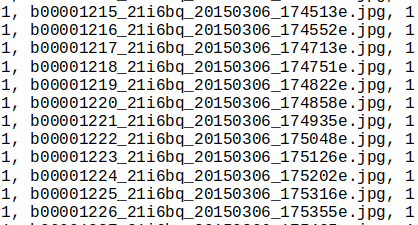
\includegraphics[scale = 0.55]{Sections/5ImageClef/images/gt_t1.png}
        \caption{Excerpt of the ground truth for the dev topic 1.}  
        \label{fig:gt}
    \end{figure}


    \subsubsection{Example of a corresponding picture}

    The dataset is composed of 200.000 images. The figure below gives an example of one of the lifelog pictures that belongs to the example topic given in section \ref{sec:devtopic1} and to the ground truth given in the figure \ref{fig:gt}:

    \begin{figure}[htb]
        \centering
        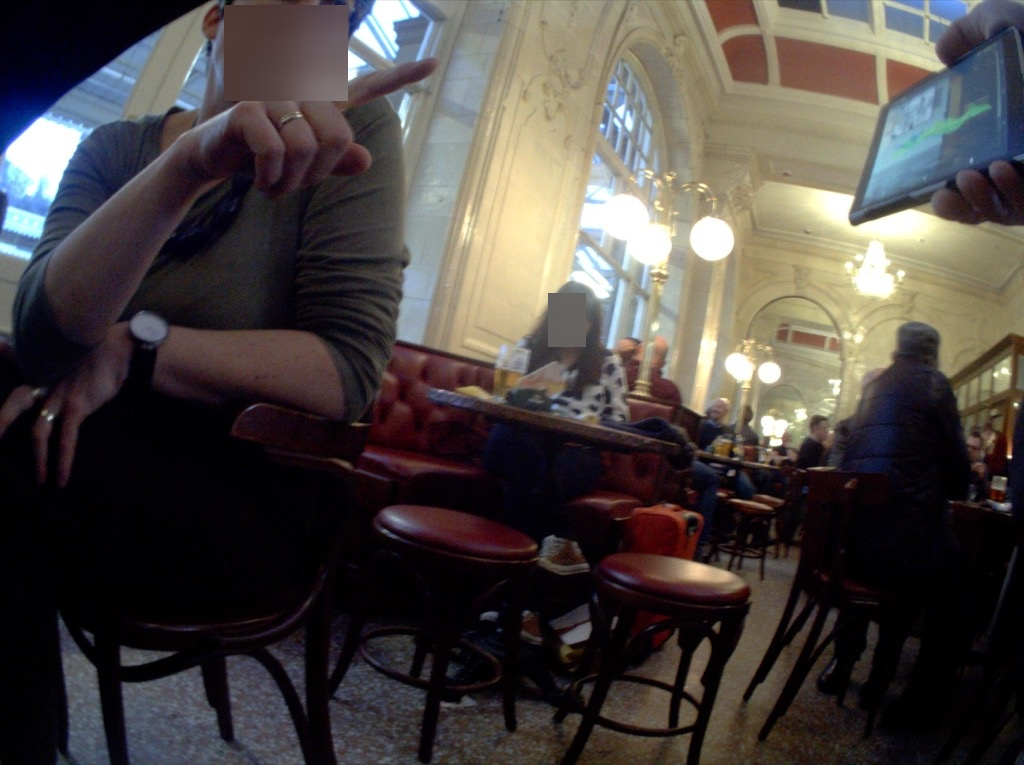
\includegraphics[scale = 0.2]{Sections/5ImageClef/images/example.png}
        \caption{Example of an image from the ground truth of the topic 1.}
    \end{figure}
    

    \newpage


    \subsection{Test Topic example}

    An example of one of the 10 textual test topics is :

        \begin{itemize}

        \item Topic 7
        

        \textbf{Title} : "Seafood at Restaurant"

        \textbf{Description} : "Find moments when u1 was eating seafood in a restaurant in the evening time"

        \textbf{Narrative} : "The moments show u1 was eating seafood in any restaurant in the evening time are considered relevant. Any dish has seafood as one of its parts is also considered relevant. Some examples of the seafood can be shrimp, lobster, salmon."

        \end{itemize}


        \subsection{Evaluation Methodology}
        \label{sec:eval}

        In order to evaluate performance, the organizers use the F1-measure at X (F1@X) evaluation method. The F1-measure is the harmonic mean of both Cluster Recall at X (CR@X) metric and the Precision at X (P@X) measure. The Cluster recall is a metric that assesses how many different clusters from the ground truth are represented among the top X results  while the Precision measures the number of  relevant photos among the top X results;

        This year edition official rankings are obtained trough the F1-measure@10, which gives equal importance to diversity (via CR@10) and relevance (via P@10). Another important aspect of a F1-measure@10 is that only the top 10 pictures for each topic with the highest confidence score are accountable for performance assessment.

    
    \newpage
    \section{Achieved Performance Results}
    \label{sec:perfomance_results}
    
    Table \ref{table:2019} and table \ref{table:2020} show the achieved performance results in different runs for different systems that were obtained in the year 2019 and 2020 for the ImageCLEFlifelog LMRT subtask. This results will be further discussed in section XX of chapter YY.
    
    \begin{table}[htb]
        
        \centering
    \begin{tabular}{ |p{4cm}|p{2.5cm}|p{2cm}|p{3cm}|  }
        \hline
        \multicolumn{4}{|c|}{\textbf{2019 Results}} \\
        \hline
        Team & System Type & Run Name & F1-measure@10 \\
        \hline
        UA.PT Bioinformatics  & automatic  & Run 1   &  0.016 \\
        UA.PT Bioinformatics  & automatic  & Run 2   &  0.026 \\
        UA.PT Bioinformatics  & automatic  & Run 3   &  0.027 \\
        UA.PT Bioinformatics  & automatic  & Run 4   &  0.027 \\
        UA.PT Bioinformatics  & automatic  & Run 5   &  0.036 \\
        UA.PT Bioinformatics  & automatic  & Run 6   &  0.057 \\
        \hline
        \multicolumn{4}{|c|}{\textbf{Best Results Achieved by a Team}} \\
        \hline
        HCMUS  & interactive  & Run 2   &  0.61 \\
        \hline        
        \end{tabular}
        \caption{Results obtained in 2019 from UA.PT Bioinformatics and the best team. }
        \label{table:2019}
    \end{table}
    \begin{table}[htb]
        \centering
    \begin{tabular}{ |p{4cm}|p{2.5cm}|p{2cm}|p{3cm}|  }   
        \hline
        \multicolumn{4}{|c|}{\textbf{2020 Results}} \\
        \hline
        Team & System Type & Run Name & F1-measure@10 \\
        \hline
        UA.PT Bioinformatics  & automatic  & Run 1   &  0.03 \\
        UA.PT Bioinformatics  & automatic  & Run 2   &  0.03 \\
        UA.PT Bioinformatics  & interactive  & Run 3  &  0.54 \\
        \hline
        \multicolumn{4}{|c|}{\textbf{Best Results Achieved by a Team}} \\
        \hline
        HCMUS  & interactive  & Run 10   &  0.81\\
        \hline       
        \end{tabular}
        \caption{Results obtained in 2020 from UA.PT Bioinformatics and the best team.}
        \label{table:2020}
    \end{table}

    From table \ref{table:2019} and table \ref{table:2020} it is already clear that having user interaction and visualization gives much better results than a fully automatic system.